\section{Tariffs and Exchange-Rate Adjustment}
\label{sec:framework}

\subsection{The bilateral benchmark}
\label{sec:bilateral}

Consider two countries, $A$ and $B$. Let $e_{AB}$ denote units of $A$'s currency per unit of $B$'s, so that a rise is a depreciation of $A$, and write $\nu\equiv\log e_{AB}$. Country $A$ levies an ad valorem tariff $\tau$ on imports from $B$.

Each country's trade balance $\TB_i$ is the value of its exports minus the value of its imports, both at border (pre-tariff) prices and both expressed in one fixed common unit of account. Tariff revenue is a domestic transfer: it is counted neither as export revenue nor as an import payment, although its rebate or other use may affect income, quantities and therefore the trade balance. In the nested-CES model of \cref{sec:nestedces} it is rebated lump-sum. Let $v_l$ denote the common-unit value of one unit of currency $l$. We select $A$ as numeraire and normalize $v_A=1$, so these trade-balance values are numerically equal to values expressed in $A$'s currency. This convention is used throughout this section and in the proof of \cref{lem:gs}, and all derivatives in this section are evaluated at the balanced baseline unless otherwise indicated.

Equilibrium with balanced trade is $\TB_A(\nu,\tau)=0$. Linearizing,
\begin{equation}
d\,\TB_A=\TB_{A\nu}\,d\nu+\TB_{A\tau}\,d\tau=0
\quad\Longrightarrow\quad
d\nu^*=-\frac{\TB_{A\tau}}{\TB_{A\nu}}\,d\tau,
\label{eq:bilat}
\end{equation}
where $\TB_{A\nu}\equiv\partial\TB_A/\partial\nu$ holds the tariff fixed and $\TB_{A\tau}\equiv\partial\TB_A/\partial\tau$ holds $\nu$ fixed. At fixed $\nu$, the tariff produces a positive trade-balance disturbance, $\TB_{A\tau}>0$, when the tariff-induced reduction in $A$'s import payments exceeds any tariff-induced reduction in its export receipts, with tariff revenue treated according to the convention above. Conditional on $\TB_{A\tau}>0$, \cref{eq:bilat} implies an appreciation if and only if $\TB_{A\nu}>0$, that is, if and only if a depreciation improves the trade balance.

To express $\TB_{A\nu}$ in elasticities, let $Q_X$ and $Q_M$ be $A$'s export and import quantities, and hold border prices fixed in the producer's currency, as in the nested-CES model, with units chosen so that each border price is one. $A$'s export receipts are then $Q_X$ and its import payments $e_{AB}Q_M$, both in $A$'s currency, so $\TB_A=Q_X-e^{\nu}Q_M$. Define
\begin{equation*}
\varepsilon_X\equiv\frac{\partial\log Q_X}{\partial\nu},\qquad
\varepsilon_M\equiv-\frac{\partial\log Q_M}{\partial\nu},
\end{equation*}
at fixed $\tau$ and at the balanced baseline. Both are positive when a depreciation raises export volume and lowers import volume. Let $X\equiv Q_X=e_{AB}Q_M$ be the common baseline border value of exports and imports. Differentiating, $\TB_{A\nu}=Q_X\varepsilon_X-e_{AB}Q_M(1-\varepsilon_M)=X(\varepsilon_X+\varepsilon_M-1)$: the $-1$ is the valuation effect of a depreciation on the payment for each imported unit. The condition $\TB_{A\nu}>0$ is therefore the Marshall--Lerner condition $\varepsilon_X+\varepsilon_M>1$. \Cref{fig:bilateral} illustrates; the parallel shift it shows is a first-order approximation around the baseline.

\begin{remark}[Robustness of the two-country result]
\label{rem:robustness}
The sign $d\nu^*/d\tau<0$ requires two conditions:
\begin{enumerate}[label=(\roman*)]
\item at fixed $\nu$, the tariff-induced fall in import payments is larger than any tariff-induced fall in export receipts, so $\TB_{A\tau}>0$;
\item the Marshall--Lerner slope is positive, $\TB_{A\nu}>0$.
\end{enumerate}
Neither condition holds in every model or under every treatment of tariff revenue. \Cref{app:online-twocountry} states sufficient conditions for each, under which $d\nu^*/d\tau<0$. In the two-country model, a tariff therefore appreciates the tariffing country's currency whenever both conditions hold. The rest of the paper shows that with three or more countries this is no longer enough.
\end{remark}

\begin{figure}[t]
\centering
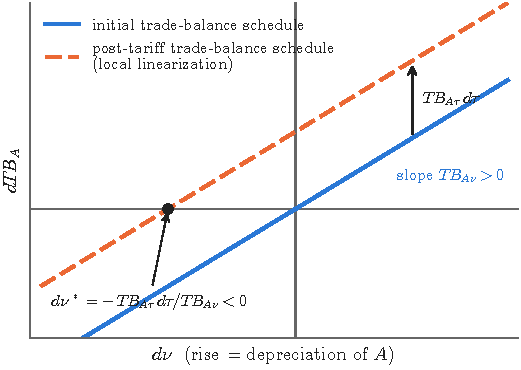
\includegraphics[width=0.65\textwidth]{fig1_bilateral.pdf}
\caption{Bilateral tariff and exchange-rate adjustment. At a fixed exchange rate, the tariff shifts the trade-balance schedule upward. When the Marshall--Lerner slope is positive, equilibrium is restored through an appreciation. Schematic.}
\label{fig:bilateral}
\end{figure}

\subsection{Multilateral adjustment}
\label{sec:representation}

Now consider $N$ countries, indexed by $\mathcal I=\{1,\dots,N\}$, and let $\mathcal I_{-A}=\mathcal I\setminus\{A\}$. Take $A$'s currency as numeraire. The $N-1$ bilateral rates $e_{Aj}$, $j\in\mathcal I_{-A}$, span all exchange-rate changes. Trade balances sum to zero (Walras' law), which leaves $N-1$ independent trade-balance conditions, indexed by $i\in\mathcal I_{-A}$:
\begin{equation*}
\TB_i\big(\{e_{Aj}\}_{j\in\mathcal I_{-A}},\{\tau_{jk}\}_{(j,k)\in\mathcal T}\big)=0,\qquad i\in\mathcal I_{-A},
\end{equation*}
where $\tau_{jk}$ is country $j$'s ad valorem tariff on imports from $k$ and $\mathcal T\equiv\{(j,k)\in\mathcal I\times\mathcal I:j\neq k\}$ is the set of all $N(N-1)$ ordered country pairs. Stack the bilateral rates as $\nu=(\nu_l)_{l\in\mathcal I_{-A}}$ with $\nu_l=\log e_{Al}$, in increasing order of $l$, and the tariffs as $\tau=(\tau_{jk})_{(j,k)\in\mathcal T}$, in lexicographic order of $(j,k)$. Linearizing,
\begin{equation}
J\,d\nu+G\,d\tau=0,\qquad J_{il}\equiv\frac{\partial\TB_i}{\partial\nu_l}\bigg|_{\tau},\qquad G_{i,(jk)}\equiv\frac{\partial\TB_i}{\partial\tau_{jk}}\bigg|_{\nu},
\label{eq:JG}
\end{equation}
for $i,l\in\mathcal I_{-A}$ and $(j,k)\in\mathcal T$, so $J\in\mathbb R^{(N-1)\times(N-1)}$ and $G\in\mathbb R^{(N-1)\times N(N-1)}$. Consider a tariff change along a fixed direction,
\begin{equation*}
d\tau=a\,ds,\qquad a\in\mathbb R^{N(N-1)},\quad\|a\|_2=1,
\end{equation*}
where the unit norm serves only to normalize the scalar $s$. Define $F\equiv Ga$, the marginal vector of trade-balance disturbances per unit increase in $s$, evaluated at unchanged exchange rates. Substituting into \cref{eq:JG},
\begin{equation*}
J\,\frac{d\nu}{ds}+Ga=0.
\end{equation*}
Provided $J$ is nonsingular, therefore,
\begin{equation}
\boxed{\;\frac{d\nu}{ds}=(-J)^{-1}F.\;}
\label{eq:response}
\end{equation}
\Cref{eq:response} separates the trade-balance effects of the tariff at unchanged exchange rates, $F$, which include expenditure switching, tariff revenue and income effects, from the exchange-rate movements required to restore external balance, $(-J)^{-1}$. In the bilateral case both are scalars, and \cref{eq:response} reduces to \cref{eq:bilat}. With $N\geq3$, however, the elements of $F$ need not have the same sign: a tariff imposed by $A$ on $B$ can improve a bystander $C$'s trade balance at unchanged exchange rates. The response of any bilateral exchange rate, including $\nu_C$, therefore depends on the full vector of tariff-induced trade-balance disturbances, not on its own element alone.

\subsection{A multilateral Marshall--Lerner condition}
\label{sec:mml}

\begin{definition}[Multilateral Marshall--Lerner condition, MML]
\label{def:mml}
Let $i,l\in\mathcal I_{-A}$. The adjustment mechanism satisfies MML if $J_{il}\geq0$ for every $l\neq i$, and $(-J)^{-1}$ exists with $(-J)^{-1}\geq0$ componentwise, that is, $[(-J)^{-1}]_{il}\geq0$ for all $i,l$. Equivalently, $-J$ is a nonsingular M-matrix.
\end{definition}

Under MML, writing $\vartheta_{ij}\equiv[(-J)^{-1}]_{ij}\geq0$,
\begin{equation}
\frac{d\nu_i}{ds}=\sum_{j\in\mathcal I_{-A}}\vartheta_{ij}F_j,\qquad i\in\mathcal I_{-A}.
\label{eq:signrule}
\end{equation}
Every disturbance enters every bilateral response with a nonnegative weight. Hence, componentwise, if $F\geq0$ then $d\nu/ds\geq0$, and if $F\leq0$ then $d\nu/ds\leq0$, where a positive $d\nu_i/ds$ is a depreciation of $A$ against $i$. This is the multilateral counterpart of the two-country result.

A primitive sufficient condition for MML is gross substitutability of trade balances, which is stated in terms of the full $N\times N$ Jacobian with respect to currency values. Let $\chi_l\equiv\log v_l$, $l\in\mathcal I$, be the log common-unit value of currency $l$. Since $e_{Aj}=v_j/v_A$,
\begin{equation*}
\nu_j=\chi_j-\chi_A,\qquad j\in\mathcal I_{-A}.
\end{equation*}
Define $\widetilde J_{il}\equiv\partial\TB_i/\partial\chi_l$ for $i,l\in\mathcal I$, at fixed tariffs. If each trade balance is homogeneous of degree one in currency values, Euler's identity gives $\sum_{l\in\mathcal I}\widetilde J_{il}=\TB_i=0$ at the balanced baseline, and Walras' law, $\sum_{i\in\mathcal I}\TB_i\equiv0$, gives $\sum_{i\in\mathcal I}\widetilde J_{il}=0$ for every $l\in\mathcal I$. Because $\chi_A$ is fixed by the normalization $v_A=1$, a change in $\nu_l$ is a change in $\chi_l$ alone, so the reduced Jacobian of \cref{eq:JG} is $J=(\widetilde J_{il})_{i,l\in\mathcal I_{-A}}$. Trade balances are gross substitutes if
\begin{equation*}
\widetilde J_{il}\geq0\qquad\text{for all }i,l\in\mathcal I,\ l\neq i,
\end{equation*}
that is, if an appreciation of currency $l$, a rise in $\chi_l$, weakly improves every other country's trade balance.

\begin{lemma}
\label{lem:gs}
If each trade balance is homogeneous of degree one in currency values, $\widetilde J_{il}\geq0$ for all $i,l\in\mathcal I$ with $l\neq i$, the reduced matrix $J=(\widetilde J_{il})_{i,l\in\mathcal I_{-A}}$ is irreducible, and $\widetilde J_{iA}>0$ for at least one $i\in\mathcal I_{-A}$, then MML holds.
\end{lemma}

\Cref{lem:gs} is the trade-balance analogue of the gross-substitutes stability results of \citet{hicks1939}, \citet{mosak1944}, \citet{metzler1945} and \citet{arrow1959}. MML ensures that multilateral adjustment is well behaved, and a disturbance vector of one sign produces exchange-rate responses of the same sign. When $F$ contains both positive and negative elements, however, MML alone does not determine the sign of an individual bilateral exchange-rate response. Positive own-exchange-rate trade-balance slopes are therefore not sufficient to sign bilateral responses in a multilateral setting.

\subsection{Symmetric trading partners}
\label{sec:decomposition}

\Cref{eq:response} holds at any balanced baseline. When the tariffing country's partners are symmetric, it can be solved using two eigenspace-specific eigenvalues of $-J$ and two of $G^{(A)}$.

Restrict attention to tariff changes imposed by $A$, $t=(t_j)_{j\in\mathcal I_{-A}}$ with $t_j\equiv d\tau_{Aj}$, and let $G^{(A)}\in\mathbb R^{(N-1)\times(N-1)}$ be the corresponding restriction of the tariff-incidence matrix,
\begin{equation*}
G^{(A)}_{ij}\equiv\frac{\partial\TB_i}{\partial\tau_{Aj}}\bigg|_{\nu},\qquad i,j\in\mathcal I_{-A},
\end{equation*}
so that $J\,d\nu+G^{(A)}t=0$. Assume that the primitives and the balanced baseline allocation are invariant to every relabeling of $A$'s $N-1$ partners. This implies that, for every $(N-1)\times(N-1)$ partner-permutation matrix $P$,
\begin{equation*}
PJP'=J\qquad\text{and}\qquad PG^{(A)}P'=G^{(A)}.
\end{equation*}
A free-trade or common-external-tariff baseline is an example only when the partner primitives are also symmetric. We then call $A$'s partners symmetric. With $\bone$ the $(N-1)$-vector of ones, decompose
\begin{equation}
t=\bar t\,\bone+\widetilde t,\qquad \bar t=\tfrac{1}{N-1}\bone't,\qquad \bone'\widetilde t=0.
\label{eq:tsplit}
\end{equation}
We call $\bar t$ \emph{average protection} and $\widetilde t$ \emph{relative treatment}. Any permutation-invariant matrix has the form $aI+b\bone\bone'$, so the one-dimensional common subspace $\operatorname{span}\{\bone\}$ and the $(N-2)$-dimensional deviation subspace $\{v:\bone'v=0\}$ are eigenspaces of both $G^{(A)}$ and $-J$:
\begin{equation*}
G^{(A)}\bone=g_S\bone,\quad G^{(A)}v=g_Dv;\qquad (-J)\bone=j_S\bone,\quad (-J)v=j_Dv\qquad(\bone'v=0).
\end{equation*}
The eigenvalues $j_D$ and $g_D$ each have multiplicity $N-2$.

We measure $A$'s effective exchange rate by its nominal effective exchange rate (NEER) with baseline bilateral trade weights. With $f_{ij}$ the border value of country $i$'s imports from $j$,
\begin{gather*}
w_{Aj}\equiv\frac{f_{Aj}+f_{jA}}{\sum_{k\neq A}(f_{Ak}+f_{kA})},\qquad \sum_{j\neq A}w_{Aj}=1,\\
E_A\equiv\prod_{j\neq A}e_{Aj}^{w_{Aj}},\qquad
d\nu^E_A\equiv d\log E_A=\sum_{j\neq A}w_{Aj}\,d\nu_j,
\end{gather*}
holding the baseline weights fixed for the local comparative static. This is the effective exchange rate throughout the paper. Under partner symmetry the bilateral trade weights are equal, $w_{Aj}=1/(N-1)$, so in this section the NEER reduces to the simple average of the bilateral log exchange rates, $d\nu^E_A=\frac{1}{N-1}\sum_{j\neq A}d\nu_j$. For partners $j,k\in\mathcal I_{-A}$ the cross rate is $e_{jk}=e_{Ak}/e_{Aj}$, units of $j$'s currency per unit of $k$'s.

\begin{proposition}[Average protection and relative treatment]
\label{prop:decomposition}
Let partners be symmetric, $N\geq3$, and $j_S,j_D\neq0$, so that $J$ is nonsingular. For any tariff vector $t$,
\begin{equation}
d\nu=\lambda_{\mathrm{avg}}\,\bar t\,\bone+\lambda_{\mathrm{rel}}\,\widetilde t,\qquad \lambda_{\mathrm{avg}}=\frac{g_S}{j_S},\quad \lambda_{\mathrm{rel}}=\frac{g_D}{j_D}.
\label{eq:decomp}
\end{equation}
Hence
\begin{equation}
d\nu^E_A=\lambda_{\mathrm{avg}}\bar t,\qquad d\nu_j-d\nu^E_A=\lambda_{\mathrm{rel}}\widetilde t_j,\qquad d\log e_{jk}=d\nu_k-d\nu_j=\lambda_{\mathrm{rel}}(t_k-t_j).
\label{eq:decompparts}
\end{equation}
Moreover, under the permutation-symmetry assumptions above, MML is equivalent to $j_S>0$ and $j_D\geq j_S$.
\end{proposition}

Average protection shifts all of $A$'s bilateral log exchange rates by the same amount, so under symmetry it determines the NEER. Relative treatment has zero mean, leaves the NEER unchanged, and moves bilateral rates around the common component; it also determines the movements in cross rates among partners. The two components lie in complementary subspaces, $\mathbb R^{N-1}=\operatorname{span}\{\bone\}\oplus\{v:\bone'v=0\}$, and each is scaled by its own coefficient. With $N=3$ these subspaces span a plane, which \cref{fig:geometry} uses to illustrate the decomposition.

\Cref{prop:decomposition} thus reduces the exchange-rate response to any tariff vector to two coefficients: $\lambda_{\mathrm{avg}}$, through which average protection moves the common component of $A$'s bilateral rates and hence its effective exchange rate, and $\lambda_{\mathrm{rel}}$, through which relative treatment moves individual bilateral rates around that component and the cross rates among partners. The decomposition follows from partner symmetry alone and does not rely on the nested-CES structure or any other particular demand system. What remains undetermined are the signs and magnitudes of $\lambda_{\mathrm{avg}}$ and $\lambda_{\mathrm{rel}}$, and hence the relative strength of the two components. \Cref{sec:nestedces} introduces a nested-CES model in which these coefficients depend on substitution between domestic and foreign goods and on substitution across foreign suppliers.
